\documentclass[12pt,fleqn]{article}\usepackage{../common}
\begin{document}
SVD ile Kumeleme

Tekil Deger Ayristirma (Singular Value Decomposition -SVD-) ile bir veri
madenciligi ornegi gorecegiz. Ornek olarak [1] adresinde tarif edilen /
paylasilan zaman serisini kullandik. Once veriyi grafikledik,

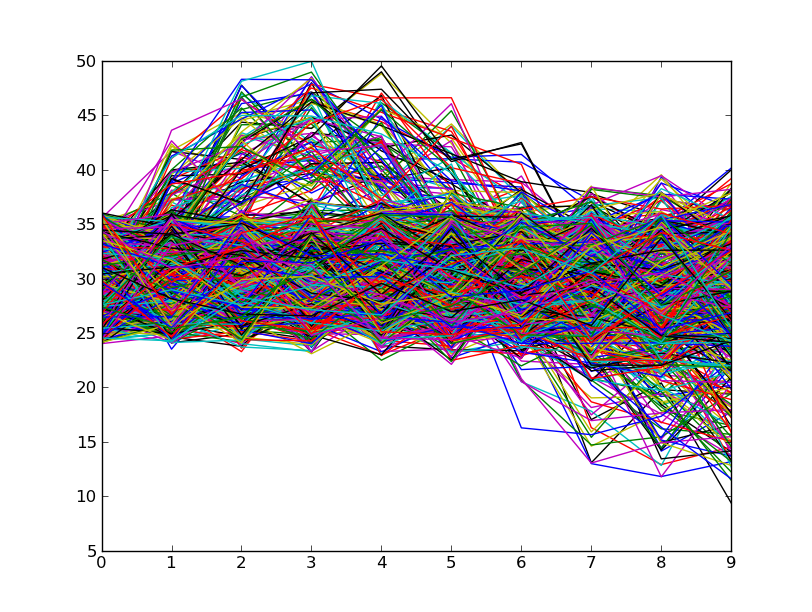
\includegraphics[height=6cm]{data.png}

Verinin tamami kullanilmadi, serinin ilk 10 noktasini aldik, ve grafige
bakinca iki tane ana seri oldugunu goruyoruz. 

\lstinputlisting[language=Python]{time1.py}

Peki bu serileri nasil otomatik olarak kumeleyerek bulurduk / birbirinden
ayirtederdik?  {\em Lineer Cebir Ders 29}'da SVD'nin matematigini
isledik. SVD bir matris $A$ uzerinde ayristirma yapar, ve $A$ herhangi
boyutta, turde bir matris olabilir.

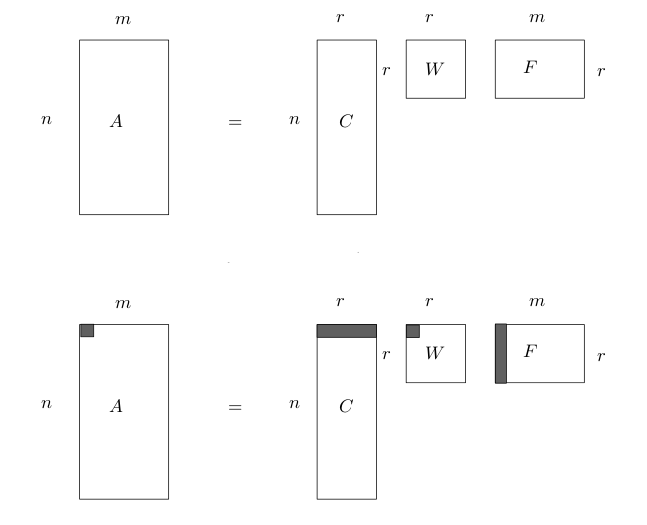
\includegraphics[height=8cm]{svd1.png}

Ayristirmanin $A=CWF$ sonucunu verir, burada $C$, ana matris ile ayni
miktarda satira sahiptir, $F$ ayni miktarda kolona sahiptir. Ayristirma
sonrasi $A$'nin kertesi (rank) ortaya cikar, eger tum $A$ kolonlari
birbirinden bagimsiz ise, o zaman $r=m$ olacaktir, ama kolonlarin bazilari
mesela ayni olcumu degisik katlarda tekrarliyor ise, o zaman matriste
tekillik vardir, ve bu durumda $r < m$ olur, ve ortadaki $W$ matrisi $r
\times r$ 
oldugu icin beklenenden daha ufak boyutlarda olabilir. 

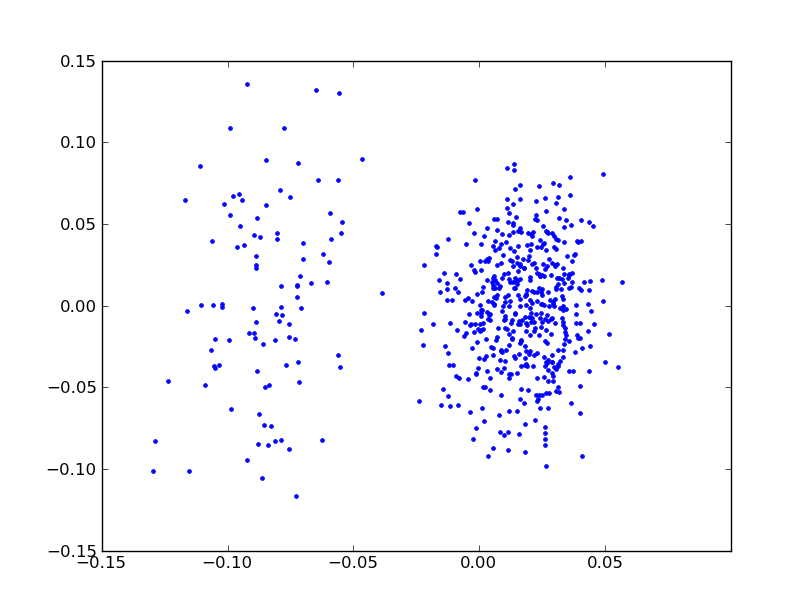
\includegraphics[height=8cm]{2d.png}

\lstinputlisting[language=Python]{time2.py}

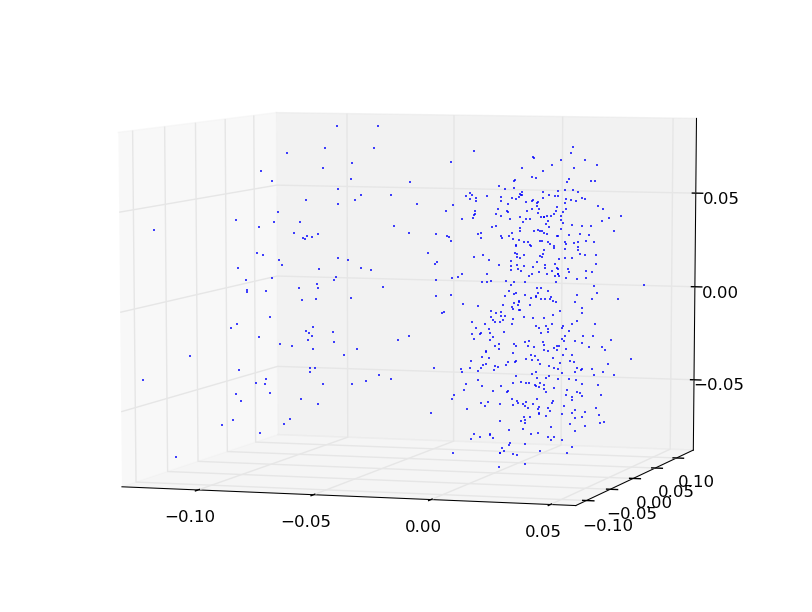
\includegraphics[height=8cm]{3d.png}

\lstinputlisting[language=Python]{time3.py}

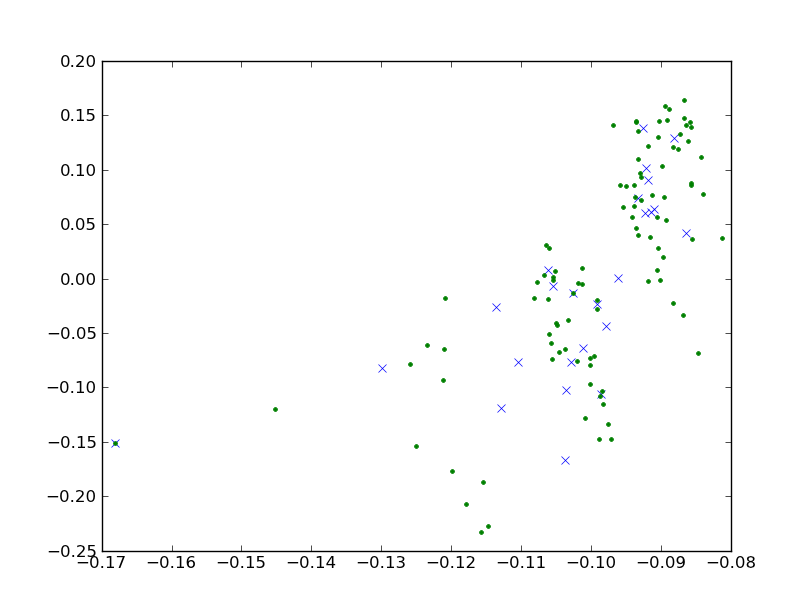
\includegraphics[height=8cm]{wordsvd.png}

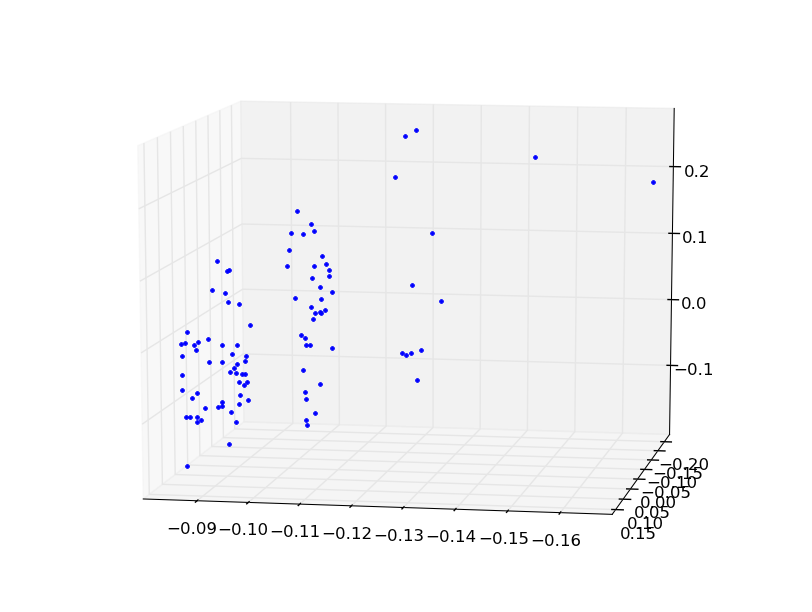
\includegraphics[height=8cm]{wordsvd3.png}

\lstinputlisting[language=Python]{wordsvd.py}


[1] http://kdd.ics.uci.edu/databases/synthetic\_control/synthetic\_control.data.html


\end{document}
